\documentclass[../main.tex]{subfiles}
\begin{document}


\section{Neuronale Netze}

\begin{figure}[h!]
  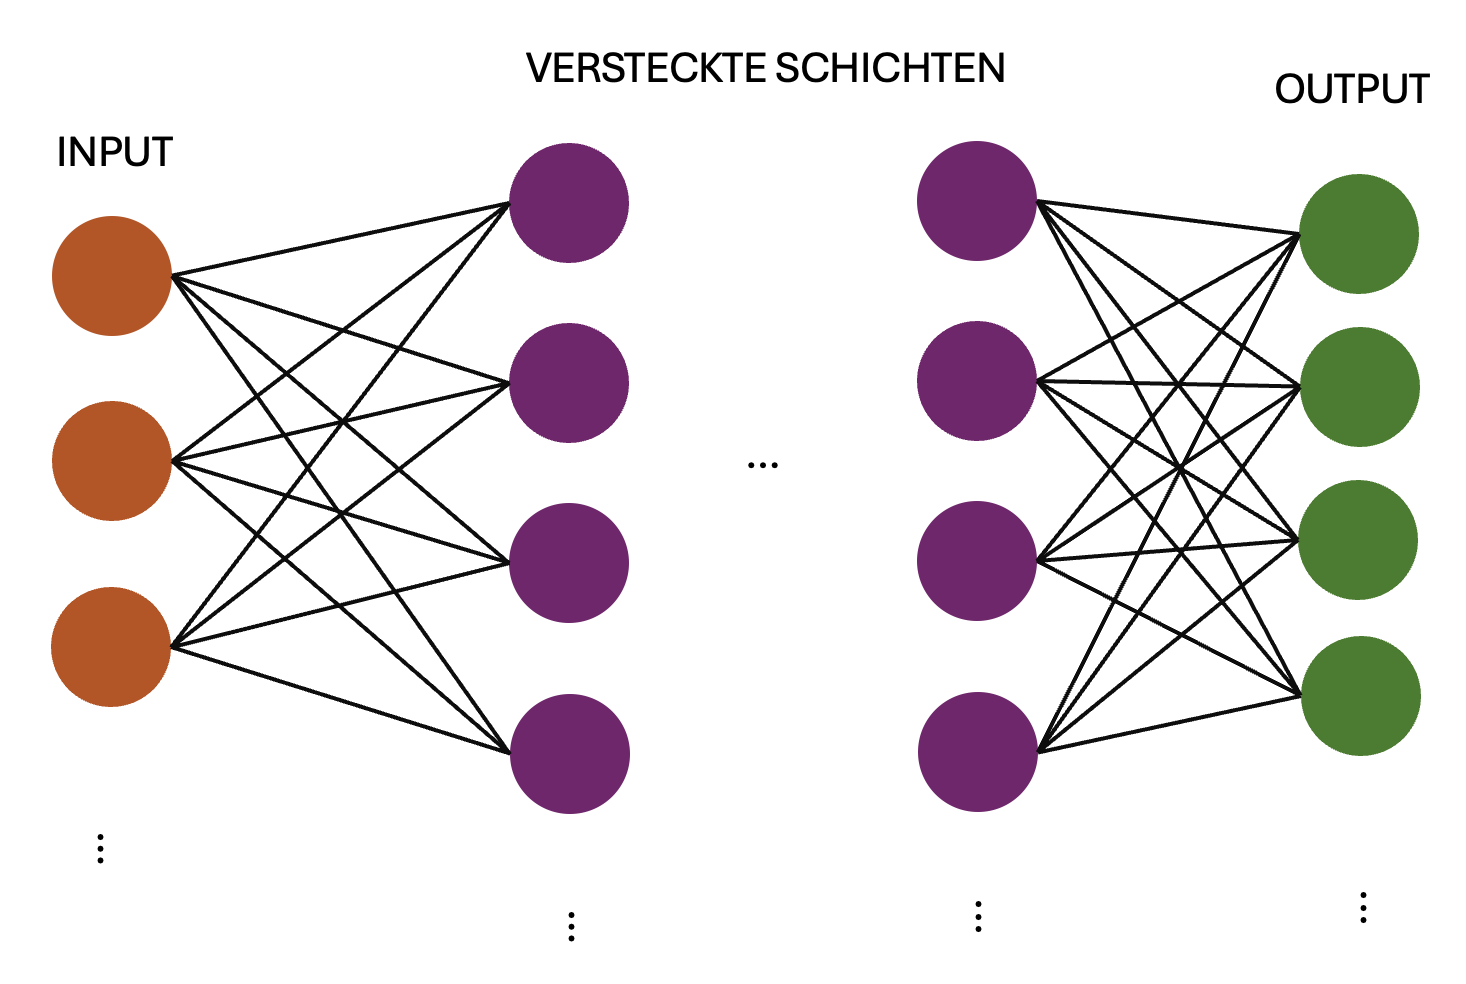
\includegraphics[scale=0.6]{bilder/NeuralNetwork.png}
  \caption{Neuronales Netzwerk}
  \label{fig:NN}
\end{figure}
\glspl{nn} bilden die Basis für \glslink{glos:ki}{KI}. Sie sind in ihrer Funktionsweise dem menschlichen Gehirn nachempfunden. Dementsprechend bestehen sie aus einer 
bestimmten Anzahl von Neuronen. Diese sind, wie in Abb \ref{fig:NN} dargestellt, in verschiedenen Schichten angeordnet. Die erste dieser Schichten wird als Eingabeschicht bezeichnet, die letzte als Ausgabeschicht. Dazwischen 
befinden sich mehrere sogenannte versteckte Schichten. Jedes Neuron ist über gewichtete Verbindungen mit allen Neuronen aus der vorherigen und der nachfolgenden Schicht verbunden. 
An jedem gegebenen Zeitpunkt hat ein Neuron einen bestimmten Wert zwischen 0 und 1, welcher dem Output des Neurons entspricht. Dieser Wert ergibt sich aus der Verarbeitung der Inputs, welche 
aus den Outputs der vorherigen Schicht berechnet werden, das heißt es wird eine Funktion auf die Summe aller Inputs ausgeführt. \\
Jede Verbindung zwischen Neuronen verfügt über eine Gewichtung zwischen -1 und 1. Diese bestimmt, mit welcher Zahl der Wert eines Neurons multipliziert wird, bevor dieser an die Neuronen in 
der folgenden Schicht weitergegeben wird. Die Gewichtungen der Verbindungen zwischen zwei Schichten können als Matrix dargestellt werden. Der Übergang von einer 
Schicht zu der darauf folgenden entspricht einer Matrixmultiplikation. \\
Die Werte der Gewichtungen stehen zu Beginn noch nicht fest. Sie werden erst durch das sogenannte Training festgelegt. Das Training eines \glslink{glos:nn}{NN} beschreibt also die konkrete Anpassung der 
Gewichtungen. Dies wird durch Backpropagation erreicht. Dafür werden die Gewichtungen zunächst mit zufälligen Werten initialisiert. Dann wird der \glslink{glos:nn}{NN}-Algorithmus mit einer Vielzahl an 
Trainingsdaten durchlaufen. Die erhaltenen werden mit den gewünschten Ergebnissen verglichen. Treten dabei zu starke Abweichungen auf, werden alle zu diesem Ergebnis beitragenden 
Gewichtungen reduziert, sodass sie weniger Einfluss auf die entstehenden Ergebnisse haben. Stimmen gewünschtes und erhaltenes Ergebnis annähernd überein, werden die dazu beitragenden 
Gewichtungen erhöht. \glslink{glos:nn}{NN}s bilden die Grundlage für weitere Technologien wie beispielsweise \glspl{llm}, welche auch für \glslink{glos:ki}{KI}-Schreibwerkzeuge verwendet werden. 

\section{Large Language Models}
\label{sec:llm}

\begin{figure}[h!]
  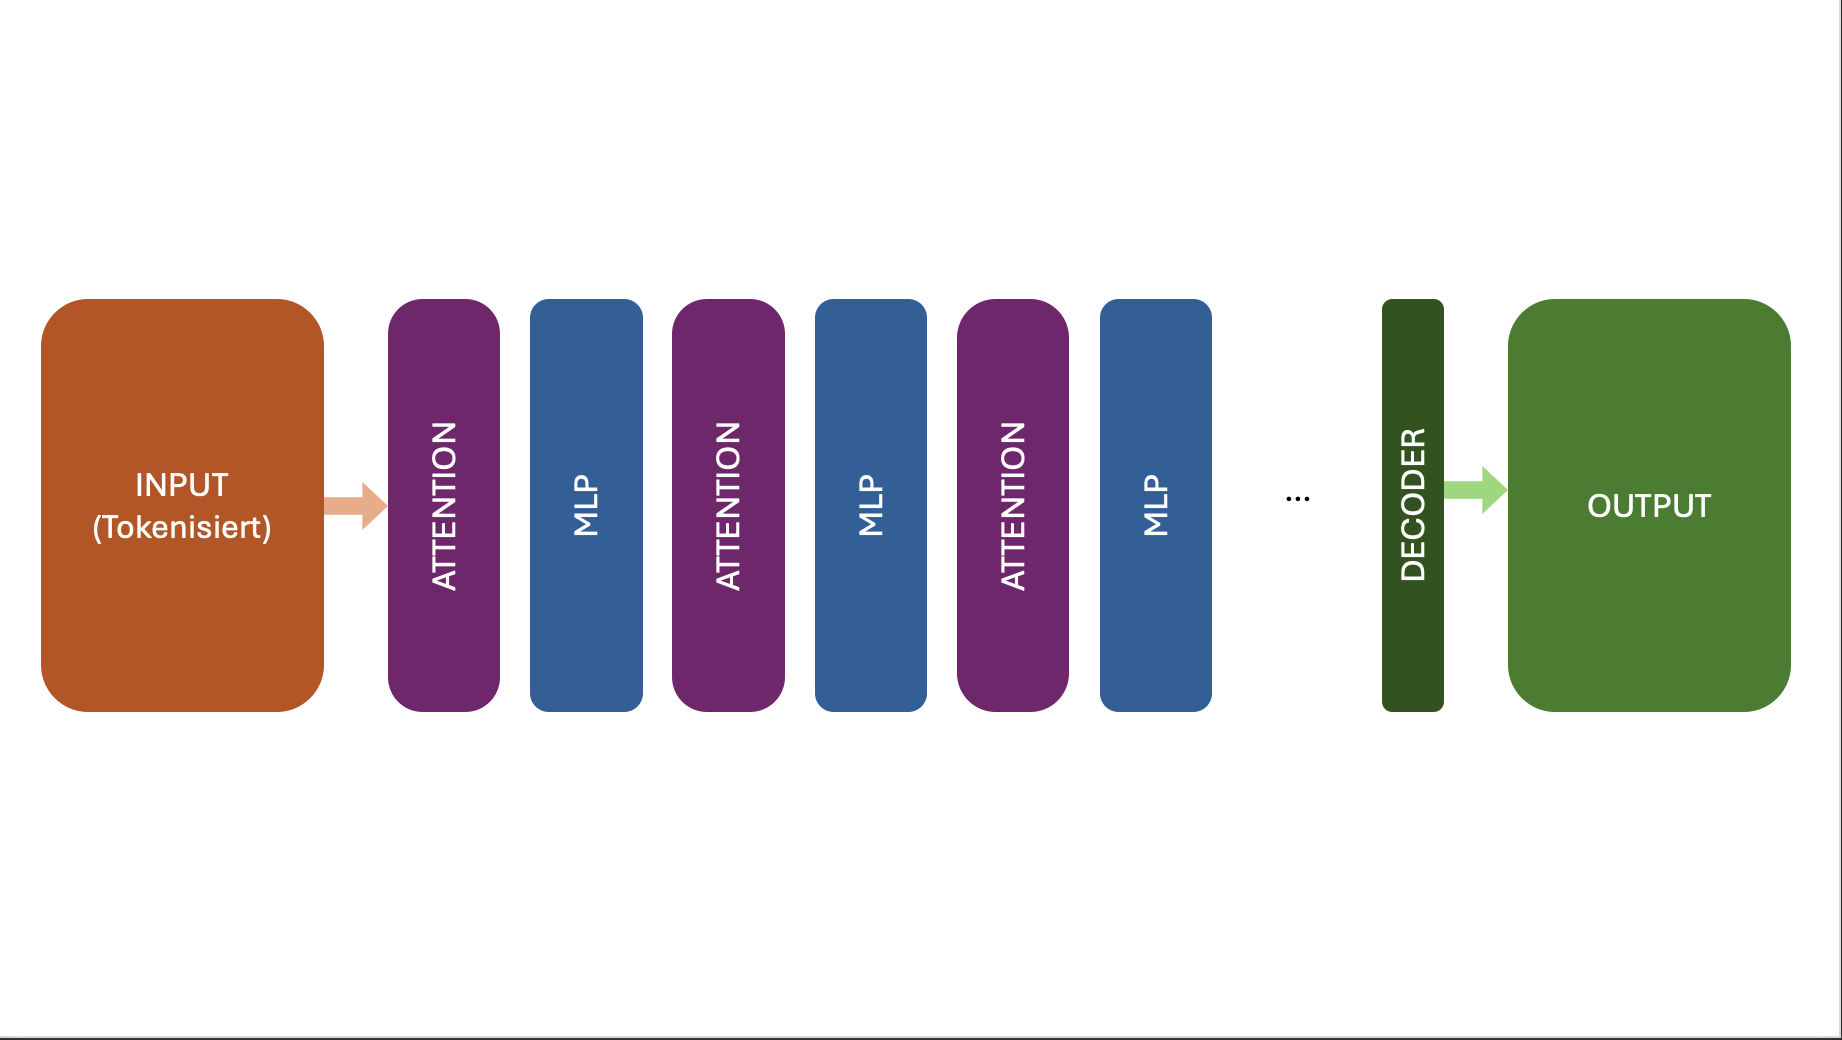
\includegraphics[scale=0.37]{bilder/Transformer.png}
  \caption{Transformer}
  \label{fig:trans}
\end{figure}
\glspl{llm} sind eine Form der \glslink{glos:ki}{KI}, welche auf natürlicher Sprache basiert. Da sie entwickelt wurden, um Texte zu generieren, werden \glspl{llm} auch als generative \glslink{glos:ki}{KI} bezeichnet.
Moderne \glslink{glos:llm}{LLM}s wie ChatGPT basieren auf einer Transformer-Architektur, welche in Abb \ref{fig:trans} schematisch dargestellt ist. Diese berechnet aus einem Eingabetext eine Wahrscheinlichkeitsverteilung 
über alle möglichen nächsten Tokens. Die Transformerarchitektur setzt sich aus folgenden Aspekten zusammen:\cite{architecture}\\

\begin{itemize}

\item \textbf{Tokenisierung:} Als erster Schritt wird der Eingabetext in einzelne Tokens unterteilt. Tokens können Wörter oder Wortteile, aber auch Satzzeichen oder einzelne Buchstaben sein. Sie sind die kleinstmögliche Einheit, welche das \glslink{glos:llm}{LLM} verarbeiten kann. Jedes Token hat eine Token-ID.\cite{architecture}

\item \textbf{Embedding:} Den Tokens werden vieldimensionale Vektoren zugeordnet. So werden sie anhand ihrer Bedeutung codiert. Die Richtungen der Vektoren im Vektorraum beinhalten semantische Bedeutungen. So liegen Wörter mit ähnlicher Bedeutung, beispielsweise Synonyme, nah beieinander.\cite{embedding}

\item \textbf{Attention:} Die einzelnen als Vektoren codierten Tokens werden durch den umliegenden Text verändert, um den Kontext des Wortes und dessen semantische Bedeutung widerzuspiegeln. Dabei werden nacheinander die einzelnen Vektoren betrachtet und ein Skalarprodukt aus dem aktuellen und jeweils den anderen Vektoren des Textes gebildet. Das Skalarprodukt beschreibt die Relevanz des anderen Tokens für die Bedeutung des aktuellen Tokens. Je größer dieser Bedeutungwert ist, desto mehr wird der aktuelle Vektor auf Grundlage des anderen Vektors verändert.\\
Die Attention-Funktion ist vollständig linear. Dieser Mechanismus lässt sich an folgendem Beispiel verdeutlichen: In den beiden Sätzen "`Ich sitze auf der Bank"' und "`Ich habe in der Bank Geld abgehoben"' hat das Wort "`Bank"' eine andere Bedeutung. Der Attention-Mechanismus passt die Vektoren, welche dieses Token codieren, so an, dass sie jeweils näher an den entsprechenden Synonymen "`Parkbank"' und "`Kreditinstitut"' liegen. Durch diese Codierung bleibt der Kontext, in welchem ein Wort verwendet wird, erhalten.\cite{attention, attention2} 

\item \textbf{\acrfull{mlp}:} Im Gegensatz zur ausschließlich linearen Attention-Funktion, kann das \glslink{glos:llm}{LLM} mithilfe des \acrshort{mlp}s auch nicht-lineare Zusammenhänge darstellen. Das \acrshort{mlp} ist ein kleines neuronales Netzwerk, meistens mit nur einer inneren Schicht sowie der Eingabe-und Ausgabeschicht. Jeder Vektor wird einmal als Input in dieses neuronale Netzwerk eingegeben und der Output zu dem ursprünglichen Vektor addiert. Mithilfe des \acrshort{mlp}s kann die Komplexität der Sprache erfasst werden.

\item \textbf{Decoder:} Die Architektur des \glslink{glos:llm}{LLM}s besteht aus mehreren Attention- und MLP-Schichten, welche abwechselnd hintereinander angeordnet sind, wie in Abb \ref{fig:trans} dargestellt wird. Abschließend verfügt es über einen Decoder, welcher den Output aus der letzten \acrshort{mlp}-Schicht als Input bekommt. Darauf wird eine Softmax-Funktion angewendet, welche eine Wahrscheinlichkeitsverteilung über alle Tokens ausgibt. Die Softmax-Funktion sorgt dafür, dass die Summe der Wahrscheinlichkeiten 1 beträgt, und jede einzelne Wahrscheinlichkeit im Intervall von 0 bis 1 liegt.\cite{architecture} 
\end{itemize}


Entsprechend der sich aus diesem Prozess ergebenden Wahrscheinlichkeitsverteilung wird in einem \glslink{glos:llm}{LLM} ein zufälliges nächstes Wort ausgewählt und an den generierten Text angefügt. 
Der Prozess wird anschließend mit dem aktualisierten Text wiederholt, sodass immer neue Tokens angefügt werden, bis eine Abbruchbedingung erreicht ist. Diese kann unter anderem das 
Erreichen der vom Nutzer festgelegten maximalen Anzahl generierter Tokens oder die Generierung eines Abbruchtokens vom \glslink{glos:llm}{LLM} selbst sein.\cite{architecture}\\

Mit dieser Architektur können erstaunliche Ergebnisse erzielt werden. Die generierten Texte ähneln menschengeschriebenen Texten sehr, wodurch sich viele Anwendungsgebiete für diese Technologie ergeben. Jedoch ergeben sich daraus auch einige Probleme und Risiken, welche im Folgenden erläutert werden sollen. 

\section{\gls{glos:prompt} und Kontext}

Um nun zu bestimmen, was für einen Text das \glslink{glos:llm}{LLM} generieren soll, erhält es einen Input. Dieser wird als \gls{glos:prompt} bezeichnet. Da \glslink{glos:ki}{KI}-Modelle verschiedene Prompts bearbeiten können, ist es 
möglich, ein Modell zum Lösen unterschiedlichster Aufgaben einzusetzen. Der Prompt setzt sich aus dem System-Prompt sowie dem User-Prompt zusammen. Zudem können noch weiteren Kontext-Angaben 
ergänzt werden.\cite{systemprompt}\\
Der System-Prompt stellt die Grundstruktur des Prompts dar und gibt dem \glslink{glos:llm}{LLM} einen grundlegenden Kontext für die Generierung des Textes mit. Zuerst wird die Information mitgeteilt, dass eine 
Frage beantwortet beziehungsweise auf eine Nutzereingabe reagiert werden soll. Darüber hinaus wird dem Modell mitgeteilt, dass es im folgenden Chat die Rolle des \glslink{glos:ki}{KI}-Assistenten übernimmt. 
Meistens werden im System-Prompt noch weitere Informationen mitgegeben, wie zum Beispiel der Stil oder Ton des Textes. Außerdem kann dem \glslink{glos:llm}{LLM} hier mitgeteilt werden, dass bestimmte Wörter 
nicht benutzt oder bestimmte Themen nicht angesprochen werden sollen, also eine erste Stufe von Filtern eingebaut werden.\cite{systemprompt}\\
Der System-Prompt wird meist durch die Entwickler des \glslink{glos:llm}{LLM}s festgelegt und ändert sich nicht. Deswegen wird er auch als "`Fixed-Prompt"' bezeichnet. Er ist für den Nutzer meist nicht sichtbar.\\
Der zweite Bestandteil des Prompts ist der User-Prompt, welcher konkret vom Nutzer eingegeben wird. Dieser kann sich bei jeder neuen Anfrage ändern und ist für den Nutzer nicht nur sichtbar, sondern 
auch veränderbar. Verändert man den Prompt, um ein besseres oder passenderes Ergebnis zu erzielen, wird dies als Prompt-Engineering bezeichnet. Um den Prompt effektiv anpassen zu können, um 
ein gewünschtes Ergebnis zu erreichen, sind oft viele Versuche nötig sowie ein tief gehendes Verständnis für die Funktionsweise des \glslink{glos:llm}{LLM}s.\cite{promptengineering}\\
Zusätzlich zum System-Prompt und User-Prompt können dem \glslink{glos:llm}{LLM} noch mehr Informationen mitgegeben werden. Die Summe aus dem Prompt und weiteren Angaben wird als Kontext bezeichnet. Dazu zählen 
zum Beispiel der vorherige Chatverlauf, damit das \glslink{glos:llm}{LLM} sich auf die vorherige Konversation beziehen kann. Auch Texte, die für die Generierung der Antwort relevant sind, können im Kontext 
übergeben werden. Ein weiteres Beispiel ist das sogenannte Few-Shot-Learning, bei dem eine  beispielhafte Konversation zwischen dem Nutzer und dem \glslink{glos:llm}{LLM} dargestellt wird, um Beispiele für das 
gewünschte Format oder den Stil der Antwort zu geben.\cite{kontext,FewShot}\\
Das Kontextfenster bezeichnet die maximale Anzahl an Tokens, die dem \glslink{glos:llm}{LLM} als Input mitgegeben werden können. Wird diese Anzahl überschritten, wird der Inhalt nicht vollständig mitgegeben, 
was zu ungewünschten und unvollständigen Ergebnissen führen kann.

\section{Wirkungen und Nebenrisiken}

\subsection{Abhängigkeit von den Trainingsdaten}

Da \glslink{glos:ki}{KI} Zusammenhänge lediglich auf Grundlage der verwendeten Trainingsdaten erlernt, sind diese häufig die Ursache für Probleme. Werden beispielsweise Trainingsdaten verwendet, 
bei denen bestimmte Personengruppen benachteiligt werden oder seltener Vorkommen, kann das die generierten Inhalte der \glslink{glos:ki}{KI} beeinflussen. Diskriminierende Inhalte können aus den Trainingsdaten 
übernommen werden. Zudem können sich durch fehlende Informationen über bestimmte Personengruppen, Sprachen, Dialekte etc. auch Nachteile in der Nutzung von \glslink{glos:ki}{KI} für betroffene 
Personengruppen ergeben.\\ Dieses Verhalten generativer \glslink{glos:ki}{KI} kann sowohl soziale als auch wirtschaftliche Folgen haben. \glslink{glos:ki}{KI} Anbieter versuchen zwar, diesem Problem durch eine möglichst 
facettenreiche Auswahl von Trainingsdaten und dem Einbau von Filtern, welche beispielsweise das Auftreten bestimmter Wörter wie Beleidigungen verhindern, diesem Problem entgegenzuwirken, 
dennoch sollten sich Nutzer diesem Risiko bewusst sein.\\

\subsection{Halluzinationen}

Die Texte, welche eine \glslink{glos:ki}{KI} ausgibt, können falsche Informationen beinhalten. Diese werden häufig als "`Halluzinationen"' bezeichnet. \glslink{glos:ki}{KI}-Halluzination beschreibt 
das Phänomen, dass generative \glslink{glos:ki}{KI}-Anwendungen Antworten erzeugen, welche zwar plausibel erscheinen, jedoch in Wirklichkeit unlogisch oder unzutreffend sind\cite{hallucinationForewarning}.\\
Halluzinationen können verschiedene Ursachen haben. Auch dafür bilden Probleme mit den Trainingsdateninhalten einen potentiellen Grund. Sind die Trainingsdaten schon älter,
können sie veraltete Informationen enthalten. Durch das Fehlen aktueller Daten kann das \glslink{glos:ki}{KI}-Modell keine korrekten Aussagen zu aktuellen Ereignissen tätigen.\\ Des 
Weiteren können die Daten ungenau, nicht fallspezifisch oder inkorrekt sein. Besonders bei einem Modelltraining mit Daten aus dem Internet besteht die Gefahr, dass 
Trainingsdaten Fehler enthalten.\\ Als weitere potenzielle Ursache für Halluzinationen kommen Schwachstellen in der Architektur in Betracht. Als "`Sycophancy"' wird das 
Phänomen beschrieben, dass das \glslink{glos:ki}{KI}-Modell Texte generiert, welche den Erwartungen des Nutzers entsprechen, ohne dabei auf fachliche Korrektheit zu achten. Dies kann ebenfalls 
durch die Formulierung des \gls{glos:prompt}s beeinflusst werden.\cite{allgemHalluzinationen} \\
Ferner birgt die Methode, mit welcher \glslink{glos:ki}{KI} Texte generiert, ein Risiko für Falschinformationen. Beispielsweise wird durch eine hohe Temperatureinstellung die 
Wahrscheinlichkeit für unplausible oder falsche Inhalte größer. Ein Artikel der Frauenhofer-Institutes beschreibt, dass gewisse Token-Typen sehr nah beieinander liegen 
und somit auch ähnliche Wahrscheinlichkeiten haben. Dazu zählten zum Beispiel "`ähnliche numerische Werte wie Preise (9,99 EUR; 10,00 EUR), nahe beieinander liegende 
Daten (2020, 2021), ähnlich klingende Namen, oder technische Begriffe und Abkürzungen (\glslink{glos:ki}{KI}, ML)"'\cite{halluzinationenFraunhofer}. Eine Verwechslung dieser Daten kann ebenfalls zu inkorrekten Aussagen 
führen.\\
Darüber hinaus können bei der Auswahl des nächsten Tokens aufgrund der Wahrscheinlichkeit, wie in \autoref{sec:llm}  beschrieben, unpassende Wörter bevorzugt werden, welche 
daraufhin die Grundlage für Halluzinationen bilden. Technisch begründet ist dieses Phänomen mit dem sogenannten Softmax-Bottleneck. Bei der Generierung der Liste von 
Wahrscheinlichkeiten für das nächste Wort wird der Softmax-Algorithmus auf einen mehrdimensionalen Vektor angewendet. Aufgrund der Natur dieses Algorithmus kann nur 
ein Ausschnitt aller möglichen Wahrscheinlichkeitsverteilungen dargestellt werden. Dadurch kann es passieren, dass die Verteilung nicht korrekt abgebildet und 
unpassenden Wörtern eine höhere Wahrscheinlichkeit zugeschrieben wird.\cite{softmax} \\
Ein so gewähltes unpassendes Wort, welches dem Text angefügt wird, bildet wiederum die Grundlage für das Generieren der darauffolgenden Wörter. Sobald in einem \glslink{glos:ki}{KI}-Chat eine 
bestimmte Falschinformation auftritt, kann die sogenannte "`Over-Confidence"' dazu führen, dass auch bei wiederholtem Nachfragen oder versuchtem Korrigieren der 
Aussage, das \glslink{glos:ki}{KI}-Modell weiterhin auf die Korrektheit der Behauptungen besteht. Dies erschwert das Überprüfen der Fakten für den Anwender.\cite{allgemHalluzinationen,softmax} \\
Selbst wenn ein \glslink{glos:ki}{KI}-generierter Text keine Falschinformationen enthält, können die beschriebenen Phänomene eine Unvollständigkeit der generierten Texte hervorrufen 
oder zu einem Abweichen von der eigentlichen Fragestellung führen.  Das als "`Instructions-Forgetting"' bekannte Phänomen beschreibt, dass eine \glslink{glos:ki}{KI} den Kontext der 
ursprünglichen Anfrage vergisst und einen Text generiert, der inhaltlich nicht der Fragestellung entspricht. Deswegen sollten \glslink{glos:ki}{KI}-generierte Texte, besonders im Kontext 
des wissenschaftlichen Schreibens, immer überprüft werden.\cite{allgemHalluzinationen}


\subsection{Erklärbarkeitsproblem}
\label{sec:erklärbarkeitsproblem}

Das Erklärbarkeitsproblem adressiert die Schwierigkeit, die Begründung für spezifische Entscheidungen \glslink{glos:ki}{KI} nachvollziehbar zu machen. Aufgrund der Funktionsweise nach dem sogenannten 
"`Black-Box"'-Prinzip ist die Rekonstruktion der kausalen Faktoren, die zu einem bestimmten Ergebnis geführt haben, limitiert. Diese Intransparenz kann die Akzeptanz und das Vertrauen in 
KI-basierte Entscheidungen beeinträchtigen. Darüber hinaus erschwert sie die Identifizierung und Korrektur von Fehlern in der zugrundeliegenden Architektur. Aktuelle Forschungsansätze 
im Bereich der "`erklärbaren KI"' zielen darauf ab, dieses Problem zu adressieren, indem sie beispielsweise Mechanismen zur Visualisierung und Darstellung des 
Entscheidungsfindungsprozesses entwickeln.\cite{explainable}
 

\subsection{Ressourcenverbrauch}

KI-Modelle verbrauchen sowohl während des Trainings als auch beim Bearbeiten der Anfragen viele Ressourcen. Desto größer das verwendete Modell, desto höher ist auch der Ressourcenverbrauch. 
Der Stromverbrauch von GPT4 0.1 liegt laut eines im Jahr 2025 veröffentlichten Artikels bei bis zu einer Kilowattstunde pro Anfrage\cite{Energieverbrauch}. Für die oben beschriebene Anpassung der Parameter sind während des Bearbeitens einer Anfrage viele 
komplexe Berechnungen in möglichst kurzer Zeit notwendig. Auch das Training ist durch die große Menge benötigter Daten und die häufig wochen- bis monatelangen Trainingszeiten 
energieintensiv. In den Rechenzentren wird zudem Wasser zur Kühlung verwendet. Der Wasser-und Ressourcenverbrauch der Nutzung eines \glslink{glos:ki}{KI}-Modells ist im Vergleich zu dem der Nutzung einer 
Suchmaschine wie Google sehr hoch\cite{KINachhaltigkeit}. 

\subsection{Datenschutz}
\label{sec:datenschutz}

Zudem besteht beim Training sowie bei der Nutzung von \glslink{glos:ki}{KI} das Problem des Datenschutzes. Die Trainingsdaten können personenbezogene Daten beinhalten. Das \glslink{glos:ki}{KI}-Modell kann bestimmte sensible 
Informationen aus den Trainingsinhalten wiedergeben, auch wenn diese nicht absichtlich gespeichert werden sollen. Einige \glslink{glos:llm}{LLM}-Anbieter behalten sich das Recht vor, das Modell anhand der 
Eingabedaten weiter zu trainieren und die Daten anderweitig zu nutzen. Auch so können personenbezogenen oder unternehmensspezifischen Informationen in die Trainings- oder Ausgabedaten 
erscheinen und so zu Datenschutzverletzungen führen. Im Falle einer missbräuchlichen Verwendung solcher Daten ist oft unklar, wer dafür die Verantwortung trägt. Vor allem bei der \glslink{glos:ki}{KI}-Nutzung 
über Online-Schnittstellen sollte daher sorgfältig mit wichtigen Informationen umgegangen werden. Sie sollten beispielsweise nicht in Form des \gls{glos:prompt}s an das Modell gegeben werden.

\end{document}